\documentclass[12pt]{exam}
\usepackage[utf8]{inputenc}

\usepackage[margin=1in]{geometry}
\usepackage{amsmath,amssymb}
\usepackage{multicol}
\usepackage[]{graphicx}
\usepackage[]{bm}
\usepackage[]{nicefrac}

\newcommand{\class}{Physique non-linéaire}
\newcommand{\term}{Master 2}
\newcommand{\examnum}{Examen final}
\newcommand{\examdate}{Février 2019}
\newcommand{\timelimit}{120 Minutes}

\pagestyle{head}
\firstpageheader{}{}{}
\runningheader{\class}{\examnum\ - Page \thepage\ of \numpages}{\examdate}
\runningheadrule


\begin{document}

\noindent
\begin{tabular*}{\textwidth}{l @{\extracolsep{\fill}} r @{\extracolsep{6pt}} l}
\textbf{\class} & \textbf{Nom -- Prénom:} & \makebox[2in]{\hrulefill}\\
% \textbf{\term} &&\\
\textbf{\examnum} &&\\
\textbf{\examdate} &&\\
% \textbf{Time Limit: \timelimit} & Teaching Assistant & \makebox[2in]{\hrulefill}
\textbf{Durée: \timelimit} &&
\end{tabular*}\\
\rule[2ex]{\textwidth}{2pt}

Ce sujet contient \numpages\ pages (en comptant la page de garde) et \numquestions\ exercices.\\
Le nombre total de point est de \numpoints.

\begin{center}
  Barême\\
  \bigskip
  \addpoints
  \gradetable[v][questions]
\end{center}

\noindent
\rule[2ex]{\textwidth}{2pt}

\begin{questions}

\question[10] \textbf{Système de fonctions itérées: la courbe de Koch}
  \noaddpoints

  \begin{figure}
    \centering
    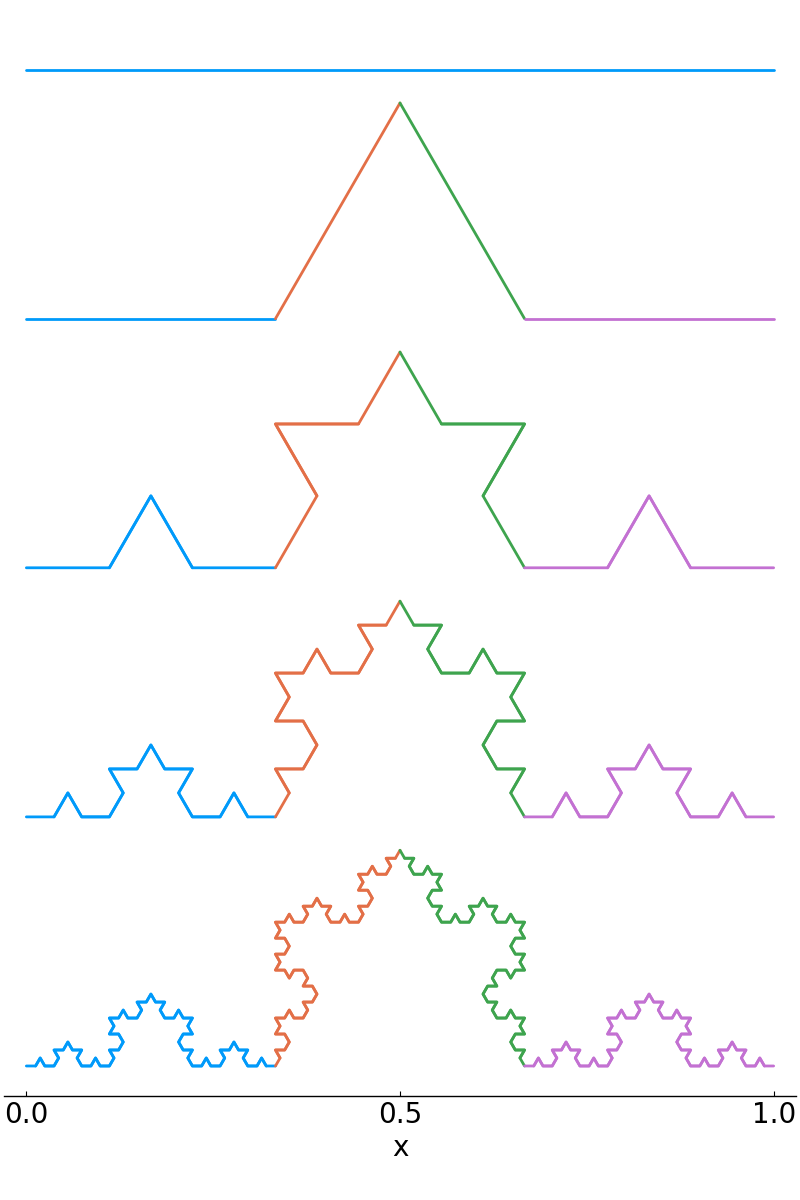
\includegraphics[height=.6\textheight]{imgs/koch_curve.png}
    \caption{Premières étapes de la construction de la courbe de Koch. \`A titre indicatif, chacun des angles d'un triangle equilatéral vaut 60$^\circ$.}
    \label{fig: koch curve}
  \end{figure}

  La construction de la courbe de Koch est décrite schématiquement sur la figure \ref{fig: koch curve} (voir page suivante). On cherche dans cet exercice à décrire cette construction à l'aide d'un système de fonctions itérées.

  \begin{parts}
    % -----> Points fixes et stabilité linéaire.
    \part[3] Donnez l'expression des quatres transformations affines $\bm{f}_i(\bm{x}) = \bm{A}_i \bm{x} + \bm{b}_i$ permettant de construire cette courbe avec $\bm{x} = (x, y)$. Expliquez en quoi consiste chacune des ces quatres transformations.
    \part[2] Montrez que chacune de ces transformations est contractante (i.e.\ les valeurs propres de chacune des matrices $\bm{A}_i$ sont comprises dans le cercle unité).
    \part[2] La courbe de Koch est la courbe limite obtenue en appliquant les transformations affines $\bm{f}_i(\bm{x})$ un nombre infini de fois. Démontrez que sa longueur est infinie.
    \part[3] Quelle est la dimension fractale de cet objet?

  \end{parts}
  \addpoints

\bigskip
\question[10] \textbf{Réduction sur la variété centrale: le système de Lorenz}
  \noaddpoints

  Considérons le système de Lorenz donné par
  \begin{equation}
    \left\{
    \begin{aligned}
      & \dot{x} = \sigma \left( y - x \right) \\
      & \dot{y} = x \left( \rho - z \right) - y \\
      & \dot{z} = - \beta z + xy.
    \end{aligned}
    \right.
    \label{eq: lorenz system}
  \end{equation}
  Dans la suite de cette exercice, on supposera que les paramètres $\sigma > 0$ et $\beta > 0$ sont fixés. L'objectif de cet exercice est de caractériser la première bifurcation rencontrée par le système.

  \medskip

  \begin{parts}
    \part On s'intéresse dans un premier temps à la stabilité du point fixe
      $$
      (x^*, y^*, z^*) = (0, 0, 0)
      $$
      pour $0 \le \rho < 1$. Pour cela, introduisons la fonction potentielle donnée par
      $$
      V(x, y, z, t) = \displaystyle \frac{x(t)^2}{\sigma} + y(t)^2 + z(t)^2 \ge 0.
      $$
      \begin{subparts}
        \subpart[2] Montrez que l'équation différentielle gouvernant la dynamique de $V$ peut être mise sous la forme suivante
        $$
        \displaystyle \frac{\mathrm{d}V}{\mathrm{d}t} = -2 \left( x - \frac{1+\rho}{2}y \right)^2 - 2 \left( 1 - \frac{(1+\rho)^2}{4} \right) y^2 - 2 \beta z^2.
        $$

        \subpart[2] Montrez que, pour $0 \le \rho < 1$, cette fonction potentielle est strictement décroissante au cours du temps.

        \subpart[1] En conclure quant à la stabilité du point fixe $(x^*, y^*, z^*) = (0, 0, 0)$. Existe-t'il d'autres attracteurs pour $0 \le \rho < 1$?
      \end{subparts}

    \part On cherche maintenant à caractériser le type de bifurcation ayant lieu pour $\rho_c = 1$. Pour cela, l'analyse se fera en deux temps.

    \begin{subparts}
      \subpart[1] Donnez l'expression de la matrice Jacobienne $\bm{J}$ du système linéarisé autour du point fixe $(x^*, y^*, z^*) = (0, 0, 0)$ et montrez que, pour $\rho = 1$, ses valeurs propres sont données par
      $$
      \lambda_1 = 0, \ \lambda_2 = -(\sigma + 1), \ \text{et } \lambda_3 = -\beta.
      $$

      \subpart[3] Afin de déterminer le type de bifurcation rencontrée, faisons le changement de variable $r = \rho - 1$ de sorte à ce que l'équation pour $y$ s'écrive
      $$
      \dot{y} = (r + 1)x - y - xz.
      $$
      La linéarisation et les valeurs propres restent les mêmes. La matrice $\bm{T}$ des vecteurs propres s'écrit par ailleurs
      $$
      \bm{T}  = \begin{bmatrix}
                    1 & \sigma & 0 \\
                    1 & -1 & 0 \\
                    0 & 0 & 1
                \end{bmatrix}.
      $$
      En introduisant le changement de variable $\bm{u} = \bm{T}^{-1} \bm{x}$, avec $\bm{x} = (x, y, z)$ et $\bm{u} = (u, v, w)$, les équations gouvernant la dynamique de $\bm{u}$ sont données par
      \begin{equation}
        \left\{
        \begin{aligned}
          & \dot{u} = \displaystyle \frac{\sigma}{1+\sigma} \left( r - w \right) \left( u + \sigma v \right) \\
          & \dot{v} = -\left( 1 + \sigma \right)v - \displaystyle \frac{1}{1+\sigma}\left( r - w \right) \left(u + \sigma v \right) \\
          & \dot{w} = -\beta w + \left( u + \sigma v \right) \left( u - v \right) \\
          & \dot{r} = 0.
        \end{aligned}
        \right.
        \label{eq: lorenz system bis}
      \end{equation}
      On peut montrer que la variété centrale $W_c$ est de la forme
      $$
      W_c = \left\{ \left(u, v, w, r \right) : v=h_1(u, r), w = h_2(u, r), h_i(0, 0) = 0, Dh_i(0, 0) = 0 \right\}.
      $$
      Supposons maintenant que
      \begin{equation}
        \begin{aligned}
          h_1(u, r) & = a_{0, 0} + a_{1, 0}u + a_{0, 1}r + a_{2, 0}u^2 + a_{1, 1}ur + a_{0, 2}r^2 + \mathcal{O}(3) \\
          h_2(u, r) & = b_{0, 0} + b_{1, 0}u + b_{0, 1}r + b_{2, 0}u^2 + b_{1, 1}ur + b_{0, 2}r^2 + \mathcal{O}(3).
        \end{aligned}
        \notag
      \end{equation}
      En déterminant les valeurs des différents coefficients $a_{i, j}$ et $b_{i, j}$, montrez que le système \eqref{eq: lorenz system bis} se réduit à un système du type
      \begin{equation}
        \left\{
        \begin{aligned}
          & \dot{u} = f(u, r) \\
          & \dot{r} = 0.
        \end{aligned}
        \right.
        \label{eq: normal form}
      \end{equation}

      \subpart[1] En se basant sur l'équation $\dot{u} = f(u, r)$ obtenue, en déduire le type de bifurcation rencontrée.
    \end{subparts}
  \end{parts}

  \bigskip

  \addpoints
  \question[10] \textbf{Théorie de Koopman}

  \medskip

  Soit le système dynamique non-linéaire suivant
  \begin{equation}
    \begin{aligned}
      \dot{x}_1 & = \mu x_1 \\
      \dot{x}_2 & = \lambda \left( x_2 - x_1^4 + 2 x_1^2 \right),
    \end{aligned}
    \label{eq: exercise 1}
  \end{equation}
  avec $\mu < 0$ et $\lambda < 0$.


  \begin{parts}
    % -----> Points fixes et stabilité linéaire.
    \noaddpoints
    \part[2] Calculez le(s) point(s) fixe(s) du système et étudiez leur stabilité linéaire.

    % -----> Variété stable.
    \noaddpoints
    \part[4] Donnez l'expression des variétés stables du point fixe situé à l'origine et tracer un schéma de l'espace des phases ainsi que quelques trajectoires.

    % -----> Théorie de Koopman.
    \noaddpoints
    \part[4] En introduisant de nouvelles variables, montrez que le système non-linéaire \eqref{eq: exercise 1} peut être ré-écrit sous la forme d'un système linéaire à 4 degrés de liberté.

    % -----> Bonus
    \noaddpoints
    \part[5 Bonus] Calculez les valeurs propres et vecteurs propres du système linéaire obtenu à la question précédente. Concluez quant aux fonctions propres de l'opérateur de Koopman.

  \end{parts}

\end{questions}

\end{document}
